\question{
    \centering
    \smallskip

    Qu'est-ce qu'une donnée fonctionnelle ?
}

Une donnée est dite fonctionnelle lorsque la variable aléatoire qui nous intéresse n'est plus une variable aléatoire à valeur dans $\mathds R^d$, comme le statisticien a l'habitude de manipuler, mais une variable aléatoire à valeur dans un espace de fonction. Concrètement, chaque réalisation n'est plus un nombre mais bien une courbe toute entière indexée (le plus souvent) sur un intervalle $\mathcal T$. 

\begin{figure}[H]
    \centering
    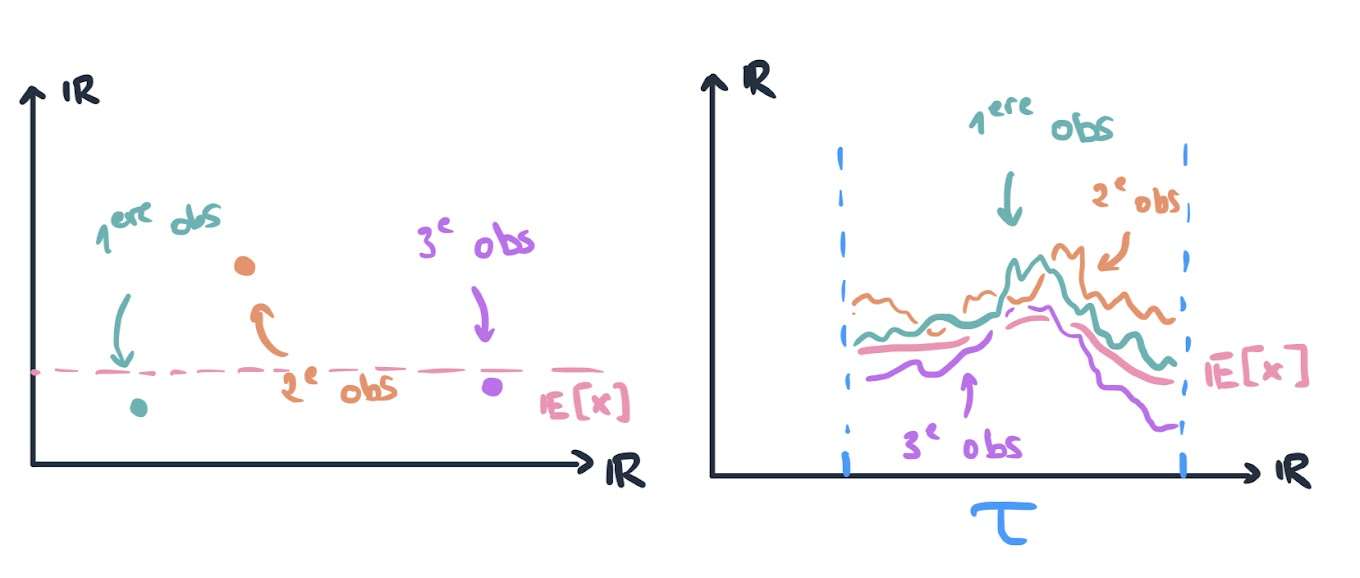
\includegraphics[width=0.7\textwidth]{Images/motivation/donneesRvsFD.jpg}
    \caption{Différence entre donnée fonctionnelle et donnée réelle}
    \label{img:RvsFD}
\end{figure}

Si le statisticien est déjà à l'aise avec l'idée qu'une variable aléatoire réelle identiquement distribuéé puisse modéliser une expérience répétable provenant d'un même phénomène, il pourra se convaincre que les données fonctionnelles permettent elles aussi de modéliser des expériences en lien (fonctionnel) avec un certain paramètre. Et c'est le lien entre les deux valeurs, cette fois-ci, qui provient d'un même phénomène. 

\largeskip

Donnons en un exemple : observons la consommation électrique d'un foyer dans une journée. Lorsque l'on travaille sur $\mathds R$, on s'intéresse à sa consommation électrique disons en l'instant $t = 12\mathsf{h}$. Formellement :
$$t \in \mathcal T \, \isdef [\, 0,24 \,[ \quad = \textsf{1 jour avec } t \textsf{ en heure}$$ 
La consommation du foyer $i$ à midi, notée $y_i$, suit la loi d'un phénomène général $Y$, comme une loi normale $\mathcal N\left( 0.27 \, \, kW\mathsf h, 0.1^2 \right)$ 
%
\footnote{ ordre de grandeur de la consommation électrique d'un foyer en France calculé à partir des données d'ENGIE disponibles librement ~\cite{engie-data-conso-moy-par-an}. \textbf{La variance est arbitraire}, tout comme le choix de la loi juste afin de servir d'exemple } 
%
par exemple. Travailler sur des données fonctionnelles dans ce cadre c'est étudier non plus la consommation $y_i$ à midi, mais regarder l'ensemble de sa consommation en même temps sur toute la journée $y_i(t) = x_i(t)$ avec $t \in \mathcal T$. 

\bigskip

On remarque ainsi que toutes les consommations électriques le long de la journée d'un foyer à l'autre suivent la même tendance : on consomme plus le matin avant le travail et le soir alors que pendant la journée on consomme moins car on est au travail. Ainsi c'est la fonction $x_i : \mathcal T \longrightarrow \mathds R$ qui suit la loi d'un phénomène $X$ général. Ce que l'on vient de dire c'est que la \textbf{relation} entre le temps $t \in \mathcal T$ et la consommation électrique ${\, y_i(t) \,}$ est elle même sujet à une loi plus générale. Grossièrement, les courbes auront la même allure, mais chaque individu a sa consommation propre.

\bigskip

\noindent 
Plus formellement : comme on a défini une variable aléatoire réelle comme une application :
$$X : \begin{array}{ccc}\Omega &\longrightarrow& \mathds R\\ \omega &\longmapsto& x = X(\omega)\end{array}$$ 

\noindent
On définit de même une donnée fonctionnelle comme une application :
$$X : \begin{array}{ccc}\Omega &\longrightarrow& \colorize{\mathcal C^0(\mathcal T, \mathds R)}\\ \omega &\longmapsto& x = X(\omega)\end{array}$$ 

\noindent
Ce que l'on observe sont donc les valeurs des paramètres $t \in \mathcal T$ ainsi que l'image de $t$ par $x$ : $y = x(t)$. Les points que le statisticien observe sont donc les couples de la forme $(t_k^{(\textsf{individu } i)}, y_k^{(\textsf{individu } i)})_{i\in \llbracket 1, m \rrbracket}$, générés par le processus aléatoire $X$ dont la réalisation est la véritable courbe $x_i$ de l'individu $i$ que l'on souhaite estimer pour travailler avec.

\bigskip

\noindent
\info{Certaines ressources sur l'analyse de données fonctionnelles définissent les données fonctionnelles de la manière suivante 
$$X : \begin{array}{ccc}\Omega \times \mathcal T &\longrightarrow& \mathds R \\ ( \omega , t ) &\longmapsto& X(\omega , t) = y\end{array}$$ 
qui selon mon humble avis, ne permet pas une interprétation clé en main du concept mais certainement plus commode à manipuler pour les mathématiciens.
}